\documentclass[10pt]{beamer}
\usetheme{PaloAlto}
\usecolortheme{default}

% ============================================================
% PACOTES
% ============================================================
\usepackage[utf8]{inputenc}
\usepackage[T1]{fontenc}
\usepackage[brazil]{babel}
\usepackage{amsmath, amsfonts, amssymb}
\usepackage{amsthm}
\usepackage{graphicx}
\usepackage{xcolor}
\usepackage{tikz}
\usetikzlibrary{arrows.meta, positioning, calc, shapes.geometric, decorations.pathreplacing}
\usepackage{csquotes}
\usepackage[style=abnt, hyperref=true]{biblatex}

% ============================================================
% ARQUIVO DE BIBLIOGRAFIA
% ============================================================
\begin{filecontents*}{referencias.bib}
@book{boaventura2009,
  author    = {Boaventura, Oswaldo and Jurkiewicz, Samuel},
  title     = {Grafos},
  publisher = {Editora Blucher},
  year      = {2009}
}
@misc{silva2020,
  author = {Da Silva, Luiz Fernando},
  title  = {Uma Proposta de Sequência Didática para o Ensino Médio: Introdução ao Estudo da Teoria dos Grafos com GeoGebra},
  year   = {2020},
  note   = {6 mai. 2020}
}
@book{cormen2009,
  author    = {Cormen, T. H. and Leiserson, C. E. and Rivest, R. L. and Stein, C.},
  title     = {Introduction to Algorithms},
  edition   = {3},
  publisher = {MIT Press},
  address   = {Cambridge, Mass.},
  year      = {2009}
}
@manual{brasil2002,
  organization = {Brasil},
  title        = {{PCN+} Ensino Médio: Orientações Educacionais Complementares aos Parâmetros Curriculares Nacionais -- Ciências da Natureza, Matemática e suas Tecnologias},
  address      = {Brasília},
  publisher    = {MEC/SEMTEC},
  year         = {2002}
}
@misc{jurkiewicz2007,
  author = {Jurkiewicz, S.},
  title  = {Grafos: Uma introdução},
  year   = {2007},
  note   = {Programa de Iniciação Científica da OBMEP 2007}
}
@mastersthesis{malta2008,
  author  = {Malta, G. H. S.},
  title   = {Grafos no ensino médio: uma inserção possível},
  school  = {Universidade Federal do Rio Grande do Sul},
  address = {Porto Alegre},
  year    = {2008}
}
@article{rodrigues2021,
  author  = {Rodrigues, A. B. and Silva, C. D.},
  title   = {O ensino de grafos e a cultura digital: novas perspectivas para a matemática escolar},
  journal = {Revista de Educação Matemática},
  volume  = {10},
  number  = {2},
  pages   = {1--15},
  year    = {2021}
}
@book{diestel2017,
  author    = {Diestel, Reinhard},
  title     = {Graph Theory},
  edition   = {5},
  publisher = {Springer},
  address   = {Berlin},
  year      = {2017}
}
@book{wilson1996,
  author    = {Wilson, Robin J.},
  title     = {Introduction to Graph Theory},
  edition   = {4},
  publisher = {Longman},
  address   = {London},
  year      = {1996}
}
@book{bondy1976,
  author    = {Bondy, J. A. and Murty, U. S. R.},
  title     = {Graph Theory with Applications},
  publisher = {North-Holland},
  address   = {New York},
  year      = {1976}
}
@book{rosen2012,
  author    = {Rosen, Kenneth H.},
  title     = {Discrete Mathematics and Its Applications},
  edition   = {7},
  publisher = {McGraw-Hill},
  address   = {New York},
  year      = {2012}
}
@article{euler1736,
  author  = {Euler, Leonhard},
  title   = {Solutio problematis ad geometriam situs pertinentis},
  journal = {Commentarii Academiae Scientiarum Imperialis Petropolitanae},
  volume  = {8},
  pages   = {128--140},
  year    = {1741},
  note    = {Apresentado em 1736}
}
@misc{brasil1996,
  author   = {Brasil},
  title    = {Lei n\textordmasculine{} 9.394, de 20 de dezembro de 1996: Estabelece as diretrizes e bases da educação nacional},
  address  = {Brasília},
  year     = {1996},
  note     = {Diário Oficial da União, Brasília, DF, 23 dez. 1996. Disponível em: \url{http://www.planalto.gov.br/ccivil_03/leis/l9394.htm}. Acesso em: 10 jan. 2026}
}
@manual{brasil2018,
  organization = {Brasil},
  title        = {Base Nacional Comum Curricular},
  address      = {Brasília},
  publisher    = {MEC},
  year         = {2018}
}
\end{filecontents*}

\addbibresource{referencias.bib}

% ============================================================
% AMBIENTES TEOREMAS EM PORTUGUÊS
% ============================================================
\newtheorem{definicao}{Definição}
\newtheorem{teorema}{Teorema}
\newtheorem{exemplo}{Exemplo}

% ============================================================
% BRASAO NA BARRA LATERAL ESQUERDA (SUPERIOR)
% ============================================================
\logo{%
    \IfFileExists{Brasão-UESC---png1.png}{
\includegraphics[width=0.9cm]{Brasão-UESC---png1.png}}{}%
}

% ============================================================
% CONFIGURACOES GERAIS
% ============================================================
\setbeamertemplate{navigation symbols}{}
\setbeamertemplate{footline}[frame number]
\setbeamertemplate{frametitle}[default][center]
\setbeamersize{text margin left=0.5cm, text margin right=0.5cm}

% ============================================================
% EFEITO DE REVELAÇÃO (INVISIBLE)
% ============================================================
\setbeamercovered{invisible}

\title[Ensino de Grafos]{PROPOSTA DE INSER\c{C}\~{A}O DO ENSINO DE GRAFOS \\ PARA ALUNOS DO ENSINO M\'{E}DIO DA REDE P\'{U}BLICA}
\author[Jos\'{e} G. D. Silva]{Jos\'{e} Guilherme Dantas Silva}
\institute[UESC]{
    Universidade Estadual de Santa Cruz \\
    Licenciatura em Matem\'{a}tica \\
    \vspace{0.2cm}
    \small Orientador: Prof. Dr. Romenique da Rocha Silva \\   \small Coorientadora: Prof\textsuperscript{a}. Ma. Sara Meira Moutta
}
\date{2026}

\begin{document}

% ============================================================
% SLIDE 1: CAPA
% ============================================================
\begin{frame}
\transglitter
\titlepage
\end{frame}

% ============================================================
% SLIDE 2: SUMARIO
% ============================================================
\begin{frame}{Sum\'{a}rio}
\transwipe 
\tableofcontents
\end{frame}

% ============================================================
% SLIDE 3: MOTIVAÇÃO (COM CORREÇÃO DE POSICIONAMENTO)
% ============================================================
\section{Motiva\c{c}\~{a}o e Problema de Pesquisa}

\begin{frame}{Motiva\c{c}\~{a}o}
\transdissolve 
\vspace*{-0.3cm} % Puxa todo o conteúdo do slide para cima
\begin{block}{O Ponto de Partida}
\begin{itemize}
    \item Estudos sobre otimiza\c{c}\~{a}o de rotas e regionaliza\c{c}\~{a}o (XXVIII ENMC).
    \item A \textbf{Teoria dos Grafos} como linguagem para modelar fen\^{o}menos reais.
    \item Distanciamento do curr\'{i}culo tradicional das demandas tecnol\'{o}gicas contempor\^{a}neas.
    \item \textcolor{red}{Crítica curricular:} A Matemática Discreta perde espaço para Álgebra e Cálculo, afastando os alunos dos problemas contemporâneos.
\end{itemize}
\end{block}
\vspace{-0.2cm} % Reduz o espaço entre os blocos, subindo a Reflexão Central
\begin{alertblock}{Reflex\~{a}o Central}
\centering
\small
\textit{``Se a Teoria dos Grafos \'{e} t\~{a}o relevante em \'{a}reas como log\'{i}stica, \\
computa\c{c}\~{a}o e redes, por que ela praticamente n\~{a}o aparece no Ensino M\'{e}dio?''}
\end{alertblock}
\end{frame}

% ============================================================
% SLIDE 4: PROBLEMA DE PESQUISA
% ============================================================
\begin{frame}{Problema de Pesquisa}
\transdissolve 
\begin{block}{Quest\~{a}o Central}
\centering
\large
Como propor a inser\c{c}\~{a}o da Teoria dos Grafos no Ensino M\'{e}dio da rede p\'{u}blica de forma contextualizada, interdisciplinar e alinhada \`{a} BNCC?
\end{block}
\vspace{0.2cm}
\begin{center}
\begin{tikzpicture}[
    node distance=1.2cm,
    box/.style={draw, rounded corners, minimum width=2.5cm, minimum height=0.9cm, align=center, font=\footnotesize}
]
    \node[box, fill=blue!15] (ctx) {Contextualiza\c{c}\~{a}o};
    \node[box, fill=green!15, right=of ctx] (inter) {Interdisciplinaridade};
    \node[box, fill=orange!15, right=of inter] (bncc) {BNCC};
    \node[box, fill=red!15, below=of inter, yshift=0.2cm] (grafos) {\textbf{Teoria dos Grafos}};
    \draw[-{Stealth}, thick] (ctx) -- (grafos);
    \draw[-{Stealth}, thick] (inter) -- (grafos);
    \draw[-{Stealth}, thick] (bncc) -- (grafos);
\end{tikzpicture}
\end{center}
\end{frame}

% ============================================================
% SLIDE 5: OBJETIVOS
% ============================================================
\section{Objetivos}

\begin{frame}{Objetivo Geral}
\transdissolve 
\begin{center}
\begin{tikzpicture}
    \node[draw, rounded corners=8pt, fill=blue!5, text width=9cm, align=center, inner sep=10pt] {
        \large
        Elaborar uma \textbf{abordagem te\'{o}rica e metodol\'{o}gica} para inserir a Teoria dos Grafos na Matem\'{a}tica do Ensino M\'{e}dio p\'{u}blico.
    };
\end{tikzpicture}
\end{center}
\vspace{0.3cm}
\begin{block}{Objetivos Espec\'{i}ficos}
\begin{itemize}
    \item Analisar o alinhamento entre Teoria dos Grafos e as compet\^{e}ncias da BNCC.
    \item Propor atividades did\'{a}ticas baseadas em Resolu\c{c}\~{a}o de Problemas.
    \item Investigar o papel da Computa\c{c}\~{a}o Desplugada no ensino de grafos.
\end{itemize}
\end{block}
\end{frame}

% ============================================================
% SLIDE 6: METODOLOGIA - ABORDAGEM E ESTRATÉGIA
% ============================================================
\section{Metodologia}

\begin{frame}{Metodologia: Abordagem e Estrat\'{e}gia}
\transdissolve 
\begin{columns}[T]
\column{0.48\textwidth}
\begin{block}{Abordagem}
Pesquisa qualitativa, car\'{a}ter bibliogr\'{a}fico e documental (BNCC, PCN+).
\end{block}
\column{0.48\textwidth}
\begin{block}{Estrat\'{e}gia Pedag\'{o}gica}
\textbf{Resolu\c{c}\~{a}o de Problemas}: o aluno como sujeito ativo, fugindo da mera transposi\c{c}\~{a}o de f\'{o}rmulas.
\end{block}
\end{columns}
\vspace{0.2cm}
\begin{alertblock}{Por que Resolu\c{c}\~{a}o de Problemas?}
\begin{itemize}
    \setlength{\itemsep}{0pt}
    \item O aluno constr\'{o}i o conhecimento a partir de situa\c{c}\~{o}es reais.
    \item Desenvolve autonomia e pensamento cr\'{i}tico.
    \item Alinha-se \`{a}s diretrizes da BNCC e do PCN+.
\end{itemize}
\end{alertblock}
\end{frame}

% ============================================================
% SLIDE 7: METODOLOGIA - ESTRUTURA DIDÁTICA
% ============================================================
\begin{frame}{Metodologia: Estrutura\c{c}\~{a}o Did\'{a}tica}
\transdissolve 
\begin{block}{Tr\^{e}s Atividades Modeladas}
\begin{itemize}
    \setlength{\itemsep}{0pt}
    \item \textbf{Planejamento Urbano} (Vila dos Grafos).
    \item \textbf{Rela\c{c}\~{o}es em Redes Sociais}.
    \item \textbf{Log\'{i}stica} (Problema do Caixeiro Viajante).
\end{itemize}
\end{block}
\vspace{0.2cm}
\begin{center}
\begin{tikzpicture}[
    node distance=1.5cm,
    phase/.style={draw, rounded corners=8pt, minimum width=2.2cm, minimum height=1cm, align=center, font=\footnotesize, fill=orange!10}
]
    \node[phase] (exp) {\textbf{Fase}\\\textbf{Explorat\'{o}ria}};
    \node[phase, right=of exp, fill=blue!10] (form) {\textbf{Fase de}\\\textbf{Formaliza\c{c}\~{a}o}};
    \node[phase, right=of form, fill=green!10] (gen) {\textbf{Fase de}\\\textbf{Generaliza\c{c}\~{a}o}};
    \draw[-{Stealth}, ultra thick, blue] (exp) -- (form);
    \draw[-{Stealth}, ultra thick, blue] (form) -- (gen);
\end{tikzpicture}
\end{center}
\vspace{0.15cm}
\begin{center}
\begin{tikzpicture}[
    node distance=0.3cm,
    desc/.style={text width=2.2cm, align=center, font=\tiny}
]
    \node[desc] at (-3.7,0) {Problema real sem teoria pr\'{e}via};
    \node[desc] at (0,0) {Alunos constroem modelos; professor introduz defini\c{c}\~{o}es};
    \node[desc] at (3.7,0) {Aplica\c{c}\~{a}o em novos cen\'{a}rios; autonomia};
\end{tikzpicture}
\end{center}
\end{frame}

% ============================================================
% SLIDE 8: FUNDAMENTAÇÃO TEÓRICA
% ============================================================
\section{Fundamenta\c{c}\~{a}o Te\'{o}rica}

\begin{frame}{Fundamenta\c{c}\~{a}o Te\'{o}rica: BNCC e Pensamento Computacional}
\transdissolve 
\begin{columns}[T]
\column{0.48\textwidth}
\onslide<2->{\begin{block}{O papel da BNCC}
\footnotesize
\begin{itemize}
    \setlength{\itemsep}{0pt}
    \item \textbf{EM13MAT315}: Algoritmos e mundo digital.
    \item \textbf{EM13MAT101}: Modelagem e depend\^{e}ncia.
    \item \textbf{EM13MAT307}: Otimiza\c{c}\~{a}o de percursos.
\end{itemize}
\end{block}}

\column{0.48\textwidth}
\onslide<3->{\begin{block}{Computa\c{c}\~{a}o Desplugada}
\footnotesize
\begin{itemize}
    \setlength{\itemsep}{0pt}
    \item Pensamento Computacional sem laborat\'{o}rios.
    \item Recursos de baixo custo (l\'{a}pis e papel).
\end{itemize}
\end{block}}
\end{columns}
\vspace{0.2cm}
\onslide<4->{\begin{alertblock}{Pensamento Computacional na BNCC}
\footnotesize
\begin{itemize}
    \setlength{\itemsep}{0pt}
    \item Decomposi\c{c}\~{a}o, Padr\~{o}es, Abstra\c{c}\~{a}o, Algoritmos.
    \item Compet\^{e}ncia transversal.
\end{itemize}
\end{alertblock}}
\end{frame}

% ============================================================
% SLIDE 9: KÖNIGSBERG - PARTE 1
% ============================================================
\section{Fundamenta\c{c}\~{a}o Matem\'{a}tica}

\begin{frame}{Contexto Histórico: O Problema das Sete Pontes de Königsberg (1736)}
\transdissolve
\begin{columns}[T]
\column{0.50\textwidth}
\large
\begin{block}{O problema histórico}
``\'{E} poss\'{i}vel atravessar todas as 7 pontes exatamente uma vez e voltar ao ponto de partida?''
\end{block}
\vspace{0.2cm}
\begin{itemize}
    \setlength{\itemsep}{0pt}
    \item A cidade de Königsberg (atual Kaliningrado) tinha 4 regiões (margens e ilhas) ligadas por 7 pontes sobre o rio Pregel.
    \item Em 1736, o matemático suíço \textbf{Leonhard Euler} publicou um artigo demonstrando a impossibilidade de tal percurso.
\end{itemize}

\column{0.48\textwidth}
\centering
\IfFileExists{Ponte de Konigsberg.png}{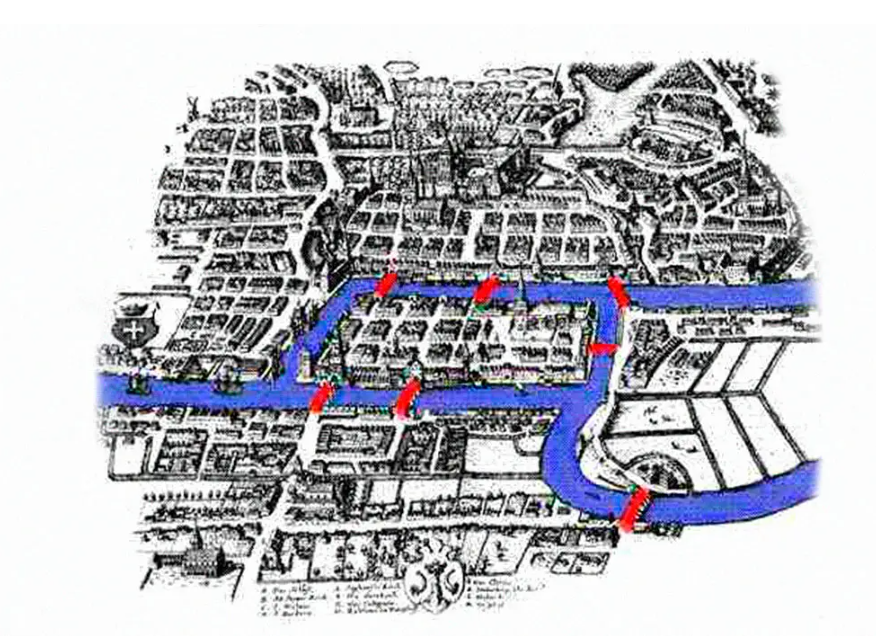
\includegraphics[width=0.8\textwidth]{Ponte de Konigsberg.png}}{\textbf{[Imagem: Ponte de Konigsberg não encontrada]}}
\vspace{0.1cm}
\textbf{Figura 1:} Mapa real das 7 pontes da cidade de Königsberg.
\end{columns}
\end{frame}

% ============================================================
% SLIDE 10: KÖNIGSBERG - PARTE 2
% ============================================================
\begin{frame}{Contexto Histórico: O Problema das Sete Pontes de Königsberg (1736)}
\transdissolve 
\begin{columns}[T]
\column{0.50\textwidth}
\begin{itemize}
    \setlength{\itemsep}{0.2cm}
    \item Euler criou uma abstração: margens/ilhas são \textbf{v\'{e}rtices} e pontes são \textbf{arestas}.
    \item Este modelo de 1736 é o \textbf{marco inicial da Teoria dos Grafos!}
\end{itemize}
\vfill
\centering
\footnotesize
\textbf{Legenda da Abstração:} \\
A e C = Margens do rio \\
B e D = Ilhas \\
Linhas = Pontes
\column{0.48\textwidth}
\centering
\begin{tikzpicture}[scale=0.6, transform shape,
    v/.style={circle, draw=black!80, fill=blue!10, very thick, minimum size=1.2cm, align=center, font=\small\bfseries},
    e/.style={draw, very thick, black!70}
]
    \node[v] (A) at (0, 2.2) {A};
    \node[v] (B) at (2.2, 0) {B};
    \node[v] (C) at (0, -2.2) {C};
    \node[v] (D) at (-2.2, 0) {D};
    \draw[e] (A) -- (B);
    \draw[e] (A) to[bend left=25] (B);
    \draw[e] (B) -- (C);
    \draw[e] (B) to[bend left=25] (C);
    \draw[e] (C) -- (D);
    \draw[e] (D) -- (A);
    \draw[e] (B) -- (D);
\end{tikzpicture}
\vspace{0.1cm}
\textbf{Figura 2:} Modelo abstrato do problema (4 Vértices, 7 Arestas).
\end{columns}
\end{frame}

% ============================================================
% SLIDE 11: O QUE É UM GRAFO?
% ============================================================
\begin{frame}{O que \'{e} um Grafo?}
\transdissolve 
\begin{columns}[T]
\column{0.55\textwidth}
\begin{definicao}[Grafo]
\small
Um grafo $G = (V, A)$, onde $V$ \'{e} um conjunto de v\'{e}rtices e $A$ \'{e} um conjunto de arestas.
\end{definicao}
\vspace{0.2cm}
\begin{exemplo}
\small
$V = \{A, B, C, D\}, \quad A = \{AB, BC, CD, DA, AC\}$
\end{exemplo}
\vspace{0.2cm}
\begin{block}{Elementos}
\small
\begin{itemize}
    \setlength{\itemsep}{0pt}
    \item \textbf{V\'{e}rtice}: modela pessoas, cidades, etc.
    \item \textbf{Aresta}: modela amizades, rotas, etc.
\end{itemize}
\end{block}
\column{0.4\textwidth}
\centering
\begin{tikzpicture}[
    scale=0.8,
    vtx/.style={circle, draw, fill=blue!15, minimum size=0.7cm, font=\small}
]
    \node[vtx] (A) at (0,0) {A};
    \node[vtx] (B) at (1.5,1) {B};
    \node[vtx] (C) at (3,0) {C};
    \node[vtx] (D) at (1.5,-1) {D};
    \draw[thick] (A) -- (B) -- (C) -- (D) -- (A);
    \draw[thick] (A) -- (C);
\end{tikzpicture}
\vspace{0.2cm}
{\scriptsize Representa\c{c}\~{a}o visual de um grafo}
\end{columns}
\end{frame}

% ============================================================
% SLIDE 12: CLASSIFICANDO GRAFOS
% ============================================================
\begin{frame}{Classificando Grafos: Tipos e Aplica\c{c}\~{o}es}
\transdissolve
\begin{columns}[T]
\column{0.32\textwidth}
\begin{block}{\footnotesize N\~{a}o Dirigido}
\footnotesize
Rela\c{c}\~{o}es sim\'{e}tricas. \\
\textbf{Ex:} WhatsApp.
\vspace{0.1cm}
\begin{center}
\begin{tikzpicture}[scale=0.6,
    vtx/.style={circle, draw, fill=red!15, minimum size=0.6cm, font=\scriptsize}
]
    \node[vtx] (a) at (0,0) {A};
    \node[vtx] (b) at (2,0) {B};
    \node[vtx] (c) at (1,1.7) {C};
    \draw[thick] (a) -- (b) -- (c) -- (a);
\end{tikzpicture}
\end{center}
\end{block}

\column{0.32\textwidth}
\begin{block}{\footnotesize Dirigido}
\footnotesize
Rela\c{c}\~{o}es assim\'{e}tricas. \\
\textbf{Ex:} Instagram.
\vspace{0.1cm}
\begin{center}
\begin{tikzpicture}[scale=0.6,
    vtx/.style={circle, draw, fill=blue!15, minimum size=0.6cm, font=\scriptsize}
]
    \node[vtx] (a) at (0,0) {A};
    \node[vtx] (b) at (2,0) {B};
    \node[vtx] (c) at (1,1.7) {C};
    \draw[-{Stealth}, thick] (a) -- (b);
    \draw[-{Stealth}, thick] (b) -- (c);
    \draw[-{Stealth}, thick] (c) -- (a);
\end{tikzpicture}
\end{center}
\end{block}

\column{0.32\textwidth}
\begin{block}{\footnotesize Ponderado}
\footnotesize
Arestas com pesos (dist\^{a}ncia). \\
\textbf{Ex:} GPS.
\vspace{0.1cm}
\begin{center}
\begin{tikzpicture}[scale=0.6,
    vtx/.style={circle, draw, fill=green!20, minimum size=0.6cm, font=\scriptsize}
]
    \node[vtx] (a) at (0,0) {A};
    \node[vtx] (b) at (2,0) {B};
    \node[vtx] (c) at (1,1.7) {C};
    \draw[thick] (a) -- node[above, font=\tiny] {5} (b);
    \draw[thick] (b) -- node[right, font=\tiny] {3} (c);
    \draw[thick] (c) -- node[left, font=\tiny] {4} (a);
\end{tikzpicture}
\end{center}
\end{block}
\end{columns}
\end{frame}

% ============================================================
% SLIDE 13: LEMA DO APERTO DE MÃO
% ============================================================
\begin{frame}{Lema do Aperto de M\~{a}o --- Demonstra\c{c}\~{a}o Geom\'{e}trica}
\transdissolve 
\begin{teorema}[Lema do Aperto de M\~{a}o]
\small
$\displaystyle\sum_{v \in V} \delta(v) = 2|A|$
\end{teorema}
\begin{columns}[T]
\column{0.5\textwidth}
\centering
\begin{tikzpicture}[scale=0.5,
    vertex/.style={circle, draw, fill=blue!10, minimum size=0.7cm, font=\small},
    edge/.style={thick}
]
    \node[vertex] (A) at (0,0) {A};
    \node[vertex] (B) at (3,0) {B};
    \node[vertex] (C) at (1.5,-2.5) {C};

    \onslide<1->{\draw[edge, gray!30] (A) -- (B);}
    \onslide<2->{\draw[edge, red, line width=1.5pt] (A) -- (B);}
    \onslide<2->{\draw[red, thick, -{Stealth}] (A) -- ++(-0.7,0.7) node[above, font=\tiny] {+1};}
    \onslide<2->{\draw[red, thick, -{Stealth}] (B) -- ++(0.7,0.7) node[above, font=\tiny] {+1};}

    \onslide<3->{\draw[edge, gray!30] (B) -- (C);}
    \onslide<4->{\draw[edge, red, line width=1.5pt] (B) -- (C);}
    \onslide<4->{\draw[red, thick, -{Stealth}] (B) -- ++(0.8,-0.4) node[right, font=\tiny] {+1};}
    \onslide<4->{\draw[red, thick, -{Stealth}] (C) -- ++(-0.8,-0.4) node[left, font=\tiny] {+1};}

    \onslide<5->{\draw[edge, gray!30] (C) -- (A);}
    \onslide<6->{\draw[edge, red, line width=1.5pt] (C) -- (A);}
    \onslide<6->{\draw[red, thick, -{Stealth}] (A) -- ++(-0.4,-0.7) node[left, font=\tiny] {+1};}
    \onslide<6->{\draw[red, thick, -{Stealth}] (C) -- ++(0.4,-0.7) node[right, font=\tiny] {+1};}

    \onslide<7->{\node[vertex, fill=yellow!30] at (A) {A};}
    \onslide<7->{\node[vertex, fill=yellow!30] at (B) {B};}
    \onslide<7->{\node[vertex, fill=yellow!30] at (C) {C};}
    \onslide<7->{\node[font=\small] at (1.5,-3.5) {\textbf{Total:} $2+2+2=6=2 \times 3$};}
\end{tikzpicture}
\column{0.48\textwidth}
\footnotesize
\begin{block}{Passo a Passo}
\begin{itemize}
    \setlength{\itemsep}{0pt}
    \item<2-> \textcolor{red}{Aresta AB}: contribui +1 para A e +1 para B.
    \item<4-> \textcolor{red}{Aresta BC}: contribui +1 para B e +1 para C.
    \item<6-> \textcolor{red}{Aresta CA}: contribui +1 para C e +1 para A.
    \item<7-> Cada aresta adiciona \textbf{+2} \`{a} soma total dos graus.
\end{itemize}
\end{block}
\end{columns}
\end{frame}

% ============================================================
% SLIDE 14: TEOREMA DE EULER
% ============================================================
\begin{frame}{Teorema de Euler --- Caminhos e Circuitos}
\transdissolve 
\begin{teorema}[Teorema de Euler]
\small
Um grafo conexo admite:
\begin{itemize}
    \setlength{\itemsep}{0pt}
    \item \textbf{Caminho Euleriano}: exatamente 2 v\'{e}rtices de grau \'{i}mpar.
    \item \textbf{Circuito Euleriano}: todos os v\'{e}rtices de grau par.
\end{itemize}
\end{teorema}
\vspace{0.2cm}
\begin{columns}[T]
\column{0.45\textwidth}
\centering
\begin{tikzpicture}[scale=0.45,
    vertex/.style={circle, draw, fill=purple!10, minimum size=0.7cm, font=\small},
    edge/.style={thick}
]
    \node[vertex] (A) at (0,0) {A};
    \node[vertex] (B) at (2.5,0) {B};
    \node[vertex] (C) at (1.25,2) {C};
    \onslide<1->{\draw[edge, gray!40] (A) -- (B);}
    \onslide<2->{\draw[edge, red, line width=1.5pt] (A) -- (B);}
    \onslide<3->{\draw[edge, gray!40] (B) -- (C);}
    \onslide<4->{\draw[edge, red, line width=1.5pt] (B) -- (C);}
    \onslide<5->{\draw[edge, gray!40] (C) -- (A);}
    \onslide<6->{\draw[edge, red, line width=1.5pt] (C) -- (A);}
    \onslide<7->{\node[vertex, fill=green!30] at (A) {A};}
    \onslide<7->{\node[vertex, fill=green!30] at (B) {B};}
    \onslide<7->{\node[vertex, fill=green!30] at (C) {C};}
    \onslide<7->{\node[font=\tiny] at (1.25,-0.8) {Grau(A)=Grau(B)=Grau(C)=2 (par)};}
    \onslide<7->{\node[font=\tiny] at (1.25,-1.3) {\textbf{Circuito Euleriano!}};}
\end{tikzpicture}
\column{0.5\textwidth}
\footnotesize
\begin{block}{Interpreta\c{c}\~{a}o}
\begin{itemize}
    \setlength{\itemsep}{0pt}
    \item<2-> Passo 1: percorrer AB.
    \item<4-> Passo 2: percorrer BC.
    \item<6-> Passo 3: percorrer CA, retornando ao in\'{i}cio!
    \item<7-> Todos os graus s\~{a}o pares $\Rightarrow$ \textbf{circuito}.
\end{itemize}
\end{block}
\end{columns}
\end{frame}

% ============================================================
% SLIDE 15: GRAFOS COMPLETOS (Kn)
% ============================================================
\begin{frame}{Grafos Completos ($K_n$) --- Constru\c{c}\~{a}o e Demonstra\c{c}\~{a}o}
\transdissolve 
\begin{definicao}[Grafo Completo]
\small
Todo par de v\'{e}rtices distintos est\'{a} ligado por exatamente uma aresta.
\end{definicao}
\vspace{0.1cm}
\begin{columns}[T]
\column{0.42\textwidth}
\centering
\begin{tikzpicture}[scale=0.5,
    vertex/.style={circle, draw, fill=green!10, minimum size=0.7cm, font=\small},
    edge/.style={thick}
]
    \node[vertex] (1) at (0,2) {1};
    \node[vertex] (2) at (2,0) {2};
    \node[vertex] (3) at (0,-2) {3};
    \node[vertex] (4) at (-2,0) {4};

    \onslide<1->{\draw[edge, gray!30] (1) -- (2);}
    \onslide<2->{\draw[edge, red, line width=1.5pt] (1) -- (2);}

    \onslide<3->{\draw[edge, gray!30] (2) -- (3);}
    \onslide<4->{\draw[edge, red, line width=1.5pt] (2) -- (3);}

    \onslide<5->{\draw[edge, gray!30] (3) -- (4);}
    \onslide<6->{\draw[edge, red, line width=1.5pt] (3) -- (4);}

    \onslide<7->{\draw[edge, gray!30] (4) -- (1);}
    \onslide<8->{\draw[edge, red, line width=1.5pt] (4) -- (1);}

    \onslide<9->{\draw[edge, gray!30] (1) -- (3);}
    \onslide<10->{\draw[edge, red, line width=1.5pt] (1) -- (3);}

    \onslide<11->{\draw[edge, gray!30] (2) -- (4);}
    \onslide<12->{\draw[edge, red, line width=1.5pt] (2) -- (4);}

    \onslide<13->{\node[vertex, fill=yellow!30] at (1) {1};}
    \onslide<13->{\node[vertex, fill=yellow!30] at (2) {2};}
    \onslide<13->{\node[vertex, fill=yellow!30] at (3) {3};}
    \onslide<13->{\node[vertex, fill=yellow!30] at (4) {4};}
\end{tikzpicture}
\vspace{0.15cm}
{\scriptsize \textbf{Construção do Grafo Completo $K_4$}}

\column{0.54\textwidth}
\scriptsize
\begin{block}{Demonstração da Fórmula $|A| = \frac{n(n-1)}{2}$}
\setlength{\itemsep}{0.15cm}
\begin{itemize}
    \item<2-> Em um grafo completo com $n$ vértices, cada vértice possui grau $\delta(v) = n-1$.
    \item<4-> A soma total dos graus é: $\displaystyle\sum_{v \in V} \delta(v) = n(n-1)$.
    \item<6-> Pelo \textbf{Lema do Aperto de Mão}: $2|A| = n(n-1)$.
    \item<8-> Logo, $\displaystyle \mathbf{|A| = \frac{n(n-1)}{2}}$.
    \item<10-> Para $n=4$: $|A| = \frac{4 \cdot 3}{2} = \mathbf{6}$ arestas.
\end{itemize}
\end{block}
\end{columns}
\end{frame}

% ============================================================
% SLIDE 16: TRANSIÇÃO DA TEORIA PARA A PRÁTICA
% ============================================================
\section{Proposta Did\'{a}tica}

\begin{frame}{Conectando a Teoria à Prática}
\transdissolve
\begin{columns}[T]
\column{0.32\textwidth}
\begin{block}{\footnotesize Fase Exploratória}
\footnotesize
Apresentação do problema real, sem teoria prévia.
\end{block}
\column{0.32\textwidth}
\begin{block}{\footnotesize Fase de Formalização}
\footnotesize
Alunos constroem modelos; professor introduz as definições formais.
\end{block}
\column{0.32\textwidth}
\begin{block}{\footnotesize Fase de Generalização}
\footnotesize
Aplicação dos conceitos em novos cenários, promovendo autonomia.
\end{block}
\end{columns}
\vspace{0.4cm}
\begin{alertblock}{O que esperar a seguir?}
\centering
\small
Ao invés de uma lista de exercícios, você verá três \textbf{situações-problema contextualizadas}, pensadas para ensinar os conceitos de forma ativa e significativa aos alunos.
\end{alertblock}
\end{frame}

% ============================================================
% SLIDE 17: PROPOSTA I - DESAFIOS (FONTES AUMENTADAS)
% ============================================================
\begin{frame}{Proposta I: A Vila dos Grafos}
\transdissolve 
\textbf{Objetivo:} Construir um grafo a partir de um contexto urbano, identificar vértices e arestas, calcular graus e verificar o Lema do Aperto de Mão.
\vspace{0.3cm}
\begin{columns}[T]
\column{0.55\textwidth}
\centering
\begin{tikzpicture}[
    scale=0.5, transform shape,
    vertex/.style={circle, draw=blue!70!black, fill=blue!10, very thick, minimum size=1.2cm, align=center, font=\footnotesize\bfseries},
    centervertex/.style={circle, draw=orange!80!black, fill=orange!20, very thick, minimum size=1.2cm, align=center, font=\footnotesize\bfseries},
    edge/.style={draw, very thick, black!70}
]
    \node[centervertex] (D) at (0,0) {D\\Praça};
    \node[vertex] (A) at (-2.5, 1.5) {A\\Pref.};
    \node[vertex] (B) at (2.5, 1.5) {B\\Escola};
    \node[vertex] (C) at (2.5, -1.5) {C\\Padaria};
    \node[vertex] (E) at (-2.5, -1.5) {E\\Hosp.};
    \draw[edge] (A) -- (B) node[midway, above, font=\scriptsize] {Rua 1};
    \draw[edge] (A) -- (D) node[midway, sloped, above, font=\scriptsize] {Rua 2};
    \draw[edge] (B) -- (C) node[midway, right, font=\scriptsize] {Rua 3};
    \draw[edge] (B) -- (D) node[midway, sloped, above, font=\scriptsize] {Rua 4};
    \draw[edge] (C) -- (D) node[midway, sloped, below, font=\scriptsize] {Rua 5};
    \draw[edge] (C) -- (E) node[midway, below, font=\scriptsize] {Rua 6};
    \draw[edge] (D) -- (E) node[midway, sloped, below, font=\scriptsize] {Rua 7};
\end{tikzpicture}
\column{0.45\textwidth}
\footnotesize
\begin{block}{Desafios}
\setlength{\itemsep}{0pt}
\begin{itemize}
    \item<+-> \textbf{Q1:} Desenhe o mapa da vila como um grafo.
    \item<+-> \textbf{Q2:} Liste os conjuntos de vértices e de arestas.
    \item<+-> \textbf{Q3:} Calcule o grau de cada vértice.
    \item<+-> \textbf{Q4:} Some os graus. Compare com o total de arestas. O que você conclui?
\end{itemize}
\end{block}
\end{columns}
\end{frame}

% ============================================================
% SLIDE 18: PROPOSTA I - GABARITO (FONTES AUMENTADAS)
% ============================================================
\begin{frame}{Gabarito da Proposta I}
\transdissolve 
\begin{columns}[T]
\column{0.55\textwidth}
\centering
\begin{tikzpicture}[
    scale=0.5, transform shape,
    vertex/.style={circle, draw=blue!70!black, fill=blue!10, very thick, minimum size=1.2cm, align=center, font=\footnotesize\bfseries},
    centervertex/.style={circle, draw=orange!80!black, fill=orange!20, very thick, minimum size=1.2cm, align=center, font=\footnotesize\bfseries},
    edge/.style={draw, very thick, black!70}
]
    \node[centervertex] (D) at (0,0) {D\\Praça};
    \node[vertex] (A) at (-2.5, 1.5) {A\\Pref.};
    \node[vertex] (B) at (2.5, 1.5) {B\\Escola};
    \node[vertex] (C) at (2.5, -1.5) {C\\Padaria};
    \node[vertex] (E) at (-2.5, -1.5) {E\\Hosp.};
    \draw[edge] (A) -- (B) node[midway, above, font=\scriptsize] {Rua 1};
    \draw[edge] (A) -- (D) node[midway, sloped, above, font=\scriptsize] {Rua 2};
    \draw[edge] (B) -- (C) node[midway, right, font=\scriptsize] {Rua 3};
    \draw[edge] (B) -- (D) node[midway, sloped, above, font=\scriptsize] {Rua 4};
    \draw[edge] (C) -- (D) node[midway, sloped, below, font=\scriptsize] {Rua 5};
    \draw[edge] (C) -- (E) node[midway, below, font=\scriptsize] {Rua 6};
    \draw[edge] (D) -- (E) node[midway, sloped, below, font=\scriptsize] {Rua 7};
\end{tikzpicture}
\column{0.45\textwidth}
\begin{block}{Gabarito Esperado}
\centering
\footnotesize
\begin{itemize}
    \setlength{\itemsep}{0pt}
    \item Graus: A=2, B=3, C=3, D=4, E=2
    \item Soma dos graus = 14; Arestas = 7
    \item \(\mathbf{14 = 2 \times 7}\) \(\rightarrow\) \textbf{Lema do Aperto de Mão verificado!}
\end{itemize}
\end{block}
\end{columns}
\end{frame}

% ============================================================
% SLIDE 19: PROPOSTA II - DESAFIOS (FONTES AUMENTADAS)
% ============================================================
\begin{frame}{Proposta II: Redes Sociais e Conectividade}
\transdissolve 
\textbf{Objetivo:} Diferenciar grafos não dirigidos de dígrafos usando a dinâmica de redes sociais.
\vspace{0.3cm}
\begin{columns}[T]
\column{0.55\textwidth}
\centering
\begin{tikzpicture}[
    scale=0.5, transform shape,
    vertex/.style={circle, draw=black!80, fill=blue!15, very thick, minimum size=1.2cm, align=center, font=\footnotesize\bfseries},
    edge/.style={draw, very thick, black!70}
]
    \node[vertex] (Ana) at (90:2.8cm) {Ana};
    \node[vertex] (Bruno) at (18:2.8cm) {Bruno};
    \node[vertex] (Carla) at (162:2.8cm) {Carla};
    \node[vertex] (Eduarda) at (-54:2.8cm) {Eduarda};
    \node[vertex] (Diego) at (-126:2.8cm) {Diego};
    \draw[edge] (Ana) -- (Bruno);
    \draw[edge] (Ana) -- (Carla);
    \draw[edge] (Bruno) -- (Diego);
    \draw[edge] (Carla) -- (Diego);
    \draw[edge] (Diego) -- (Eduarda);
    \draw[edge] (Bruno) -- (Eduarda);
\end{tikzpicture}
\column{0.45\textwidth}
\footnotesize
\begin{block}{Desafios}
\setlength{\itemsep}{0pt}
\begin{itemize}
    \item<+-> \textbf{Q1:} Represente a rede de amizades como um grafo não dirigido e calcule os graus.
    \item<+-> \textbf{Q2:} Represente a rede de seguidores como um dígrafo. Calcule grau de entrada e saída.
    \item<+-> \textbf{Q3:} Qual modelo é melhor para um app de mensagens (WhatsApp)? Justifique.
\end{itemize}
\end{block}
\end{columns}
\end{frame}

% ============================================================
% SLIDE 20: PROPOSTA II - GABARITO (FONTES AUMENTADAS)
% ============================================================
\begin{frame}{Gabarito da Proposta II}
\transdissolve 
\begin{columns}[T]
\column{0.55\textwidth}
\centering
\begin{tikzpicture}[
    scale=0.5, transform shape,
    vertex/.style={circle, draw=black!80, fill=blue!15, very thick, minimum size=1.2cm, align=center, font=\footnotesize\bfseries},
    edge/.style={draw, very thick, black!70}
]
    \node[vertex] (Ana) at (90:2.8cm) {Ana};
    \node[vertex] (Bruno) at (18:2.8cm) {Bruno};
    \node[vertex] (Carla) at (162:2.8cm) {Carla};
    \node[vertex] (Eduarda) at (-54:2.8cm) {Eduarda};
    \node[vertex] (Diego) at (-126:2.8cm) {Diego};
    \draw[edge] (Ana) -- (Bruno);
    \draw[edge] (Ana) -- (Carla);
    \draw[edge] (Bruno) -- (Diego);
    \draw[edge] (Carla) -- (Diego);
    \draw[edge] (Diego) -- (Eduarda);
    \draw[edge] (Bruno) -- (Eduarda);
\end{tikzpicture}
\column{0.45\textwidth}
\begin{block}{Gabarito Esperado}
\footnotesize
\begin{itemize}
    \setlength{\itemsep}{0pt}
    \item \textbf{Q1:} Grafo sem setas (amizade mútua)
    \item \textbf{Q2:} Dígrafo com setas (seguidor \(\to\) seguido)
    \item \textbf{Q3:} WhatsApp usa grafo \textbf{não dirigido} (adição mútua)
\end{itemize}
\end{block}
\end{columns}
\end{frame}

% ============================================================
% SLIDE 21: PROPOSTA III - DESAFIOS (FONTES AUMENTADAS)
% ============================================================
\begin{frame}{Proposta III: O Problema do Caixeiro Viajante}
\transdissolve 
\textbf{Objetivo:} Introduzir a otimização em grafos ponderados e o conceito de explosão combinatória.
\vspace{0.3cm}
\begin{columns}[T]
\column{0.55\textwidth}
\centering
\begin{tikzpicture}[
    scale=0.5, transform shape,
    vertex/.style={circle, draw=black!80, fill=green!15, very thick, minimum size=1.2cm, align=center, font=\footnotesize\bfseries},
    edge/.style={draw, very thick, black!70},
    weight/.style={fill=white, inner sep=1pt, font=\scriptsize\bfseries, text=blue!80!black}
]
    \node[vertex] (Alfa) at (0,4) {Alfa};
    \node[vertex] (Beta) at (5,4) {Beta};
    \node[vertex] (Gama) at (0,0) {Gama};
    \node[vertex] (Delta) at (5,0) {Delta};
    \draw[edge] (Alfa) -- node[weight] {10 km} (Beta);
    \draw[edge] (Alfa) -- node[weight, pos=0.25] {15 km} (Gama);
    \draw[edge] (Beta) -- node[weight] {25 km} (Delta);
    \draw[edge] (Gama) -- node[weight] {30 km} (Delta);
    \draw[edge] (Alfa) -- node[weight, pos=0.25] {20 km} (Delta);
    \draw[edge] (Beta) -- node[weight, pos=0.25] {35 km} (Gama);
\end{tikzpicture}
\column{0.45\textwidth}
\footnotesize
\begin{block}{Desafios}
\setlength{\itemsep}{0pt}
\begin{itemize}
    \item<+-> \textbf{Q1:} Construa um grafo completo com as distâncias.
    \item<+-> \textbf{Q2:} Liste todas as rotas possíveis partindo de Alfa. Quantas são?
    \item<+-> \textbf{Q3:} Calcule o custo de cada rota. Qual é a mais curta?
    \item<+-> \textbf{Q4:} E se fossem 10 cidades (\(9!\) rotas)? O que isso revela sobre o problema?
\end{itemize}
\end{block}
\end{columns}
\end{frame}

% ============================================================
% SLIDE 22: PROPOSTA III - GABARITO (FONTES AUMENTADAS)
% ============================================================
\begin{frame}{Gabarito da Proposta III}
\transdissolve 
\begin{columns}[T]
\column{0.55\textwidth}
\centering
\begin{tikzpicture}[
    scale=0.5, transform shape,
    vertex/.style={circle, draw=black!80, fill=green!15, very thick, minimum size=1.2cm, align=center, font=\footnotesize\bfseries},
    edge/.style={draw, very thick, black!70},
    weight/.style={fill=white, inner sep=1pt, font=\scriptsize\bfseries, text=blue!80!black}
]
    \node[vertex] (Alfa) at (0,4) {Alfa};
    \node[vertex] (Beta) at (5,4) {Beta};
    \node[vertex] (Gama) at (0,0) {Gama};
    \node[vertex] (Delta) at (5,0) {Delta};
    \draw[edge] (Alfa) -- node[weight] {10 km} (Beta);
    \draw[edge] (Alfa) -- node[weight, pos=0.25] {15 km} (Gama);
    \draw[edge] (Beta) -- node[weight] {25 km} (Delta);
    \draw[edge] (Gama) -- node[weight] {30 km} (Delta);
    \draw[edge] (Alfa) -- node[weight, pos=0.25] {20 km} (Delta);
    \draw[edge] (Beta) -- node[weight, pos=0.25] {35 km} (Gama);
\end{tikzpicture}
\column{0.45\textwidth}
\begin{block}{Gabarito Esperado}
\footnotesize
\begin{itemize}
    \setlength{\itemsep}{0pt}
    \item Rota mais curta: Alfa \(\to\) Beta \(\to\) Delta \(\to\) Gama \(\to\) Alfa
    \item Custo: \(10+25+30+15 = \mathbf{80 \text{ km}}\)
    \item \(9! = 362.880\) rotas. \textbf{Explosão combinatória!}
\end{itemize}
\end{block}
\end{columns}
\end{frame}

% ============================================================
% SLIDE 23: O PAPEL DO PIBID E A REALIDADE ESCOLAR
% ============================================================
\section{O Contexto de Implementação}

\begin{frame}{O Desafio da Implementação: O PIBID e a Realidade Escolar}
\transdissolve
\begin{block}{O Objetivo de Viabilizar a Inovação na Rede Pública}
\scriptsize
\begin{itemize}
    \setlength{\itemsep}{0pt}
    \item \textbf{Dificuldades estruturais:} Falta de laboratórios de informática, turmas numerosas e currículos engessados.
    \item \textbf{Sobrecarga docente:} Professores do Ensino Médio, muitas vezes, não dispõem de tempo hábil para planejar atividades investigativas complexas.
\end{itemize}
\end{block}
\vspace{0.1cm}
\begin{alertblock}{A Vivência Prática como Pibidiano: A Solução Encontrada}
\scriptsize
\begin{itemize}
    \setlength{\itemsep}{0pt}
    \item A presença do \textbf{pibidiano na escola pública} oferece o suporte logístico e pedagógico necessário para viabilizar projetos como este.
    \item O planejamento conjunto entre professor e pibidiano e a interação direta com as turmas permitem que a pesquisa acadêmica seja efetivamente traduzida em prática de sala de aula.
    \item \textbf{Conclusão prática:} A aplicação de metodologias ativas no Ensino Médio não é uma utopia, mas uma realidade possível quando há suporte institucional e vivência prática da Iniciação à Docência.
\end{itemize}
\end{alertblock}
\end{frame}

% ============================================================
% SLIDE 24: SÍNTESE E APLICAÇÕES PRÁTICAS
% ============================================================
\section{Considera\c{c}\~{o}es Finais}

\begin{frame}{S\'{i}ntese e Aplica\c{c}\~{o}es Pr\'{a}ticas}
\transdissolve
\begin{block}{Di\'{a}logo com a BNCC e o Pensamento Computacional}
\footnotesize
\begin{itemize}
    \setlength{\itemsep}{0pt}
    \item<2-> Alinham-se \`{a} BNCC (Algoritmos, Modelagem, Otimiza\c{c}\~{a}o).
    \item<3-> Pensamento Computacional (Decomposi\c{c}\~{a}o, Abstra\c{c}\~{a}o, Algoritmos).
    \item<4-> Computa\c{c}\~{a}o Desplugada (Democratiza\c{c}\~{a}o do acesso).
\end{itemize}
\end{block}
\vspace{0.2cm}
\begin{block}{Mensagem Central}
\onslide<5->{
\centering
\small
A \textbf{Teoria dos Grafos} \'{e} uma possibilidade poderosa de aproximar a Matem\'{a}tica escolar dos \textbf{problemas do mundo contempor\^{a}neo}.
}
\end{block}
\end{frame}

% ============================================================
% SLIDES 25 E 26: REFERÊNCIAS
% ============================================================
\section*{Referências Selecionadas}

\begin{frame}{Referências Selecionadas (Parte 1)}
\transdissolve 
\footnotesize
\begin{itemize}
    \setlength{\itemsep}{0.35cm}
    \item BRASIL. \textbf{Base Nacional Comum Curricular}. MEC, 2018.
    \item BRASIL. \textbf{PCN+ Ensino Médio}. MEC/SEMTEC, 2002.
    \item EULER, L. Solutio problematis... \textit{Comm. Acad. Sci. Petrop.}, 1741.
    \item DIESTEL, R. \textbf{Graph Theory}. 5. ed. Springer, 2017.
    \item CORMEN, T. H. et al. \textbf{Introduction to Algorithms}. 3. ed. MIT Press, 2009.
    \item BOAVENTURA, O.; JURKIEWICZ, S. \textbf{Grafos}. Blucher, 2009.
\end{itemize}
\end{frame}

\begin{frame}{Referências Selecionadas (Parte 2)}
\transdissolve 
\footnotesize
\begin{itemize}
    \setlength{\itemsep}{0.35cm}
    \item WILSON, R. J. \textbf{Introduction to Graph Theory}. 4. ed. Longman, 1996.
    \item ROSEN, K. H. \textbf{Discrete Mathematics and Its Applications}. 7. ed. McGraw-Hill, 2012.
    \item MALTA, G. H. S. \textbf{Grafos no ensino médio: uma inserção possível}. UFRGS, 2008.
    \item RODRIGUES, A. B.; SILVA, C. D. O ensino de grafos e a cultura digital... \textit{Rev. Educ. Matemática}, 2021.
    \item JURKIEWICZ, S. \textbf{Grafos: Uma introdução}. OBMEP, 2007.
    \item SILVA, L. F. \textbf{Introdução ao Estudo da Teoria dos Grafos com GeoGebra}. 2020.
\end{itemize}
\end{frame}

% ============================================================
% SLIDE 27: AGRADECIMENTOS
% ============================================================
\begin{frame}[plain]
\transglitter 
\begin{center}
\vspace{1.5cm}
{\Huge \textbf{Muito Obrigado!}}

\end{center}
\end{frame}

\end{document}